%%%%%%%%%%%%%%%%%%%%%%%%%%%%%%%%%%%%%%%%%
% Article EcoFoG
% Version 2.1 (23/10/2017)
%
% adapté de :
% Stylish Article
% LaTeX Template
% Version 1.0 (31/1/13)
%
% This template has been downloaded from:
% http://www.LaTeXTemplates.com
%
% Original author:
% Mathias Legrand (legrand.mathias@gmail.com)
%
% License:
% CC BY-NC-SA 3.0 (http://creativecommons.org/licenses/by-nc-sa/3.0/)
%
%%%%%%%%%%%%%%%%%%%%%%%%%%%%%%%%%%%%%%%%%


%----------------------------------------------------------------------------------------
%	PACKAGES AND OTHER DOCUMENT CONFIGURATIONS
%----------------------------------------------------------------------------------------

\documentclass[fleqn,10pt]{ArtEcoFoG} % Document font size and equations flushed left

\setcounter{tocdepth}{3} % Show only three levels in the table of contents section: sections, subsections and subsubsections


% Pandoc environments
\usepackage{framed}
\usepackage{fancyvrb}
\providecommand{\tightlist}{%
  \setlength{\itemsep}{0pt}\setlength{\parskip}{0pt}}
\newcommand{\VerbBar}{|}
\newcommand{\VERB}{\Verb[commandchars=\\\{\}]}
\DefineVerbatimEnvironment{Highlighting}{Verbatim}{commandchars=\\\{\}, fontsize=\scriptsize} % Code R
\definecolor{shadecolor}{RGB}{248,248,248}
\newenvironment{Shaded}{\begin{snugshade}}{\end{snugshade}}
\newcommand{\KeywordTok}[1]{\textcolor[rgb]{0.13,0.29,0.53}{\textbf{{#1}}}}
\newcommand{\DataTypeTok}[1]{\textcolor[rgb]{0.13,0.29,0.53}{{#1}}}
\newcommand{\DecValTok}[1]{\textcolor[rgb]{0.00,0.00,0.81}{{#1}}}
\newcommand{\BaseNTok}[1]{\textcolor[rgb]{0.00,0.00,0.81}{{#1}}}
\newcommand{\FloatTok}[1]{\textcolor[rgb]{0.00,0.00,0.81}{{#1}}}
\newcommand{\ConstantTok}[1]{\textcolor[rgb]{0.00,0.00,0.00}{{#1}}}
\newcommand{\CharTok}[1]{\textcolor[rgb]{0.31,0.60,0.02}{{#1}}}
\newcommand{\SpecialCharTok}[1]{\textcolor[rgb]{0.00,0.00,0.00}{{#1}}}
\newcommand{\StringTok}[1]{\textcolor[rgb]{0.31,0.60,0.02}{{#1}}}
\newcommand{\VerbatimStringTok}[1]{\textcolor[rgb]{0.31,0.60,0.02}{{#1}}}
\newcommand{\SpecialStringTok}[1]{\textcolor[rgb]{0.31,0.60,0.02}{{#1}}}
\newcommand{\ImportTok}[1]{{#1}}
\newcommand{\CommentTok}[1]{\textcolor[rgb]{0.56,0.35,0.01}{\textit{{#1}}}}
\newcommand{\DocumentationTok}[1]{\textcolor[rgb]{0.56,0.35,0.01}{\textbf{\textit{{#1}}}}}
\newcommand{\AnnotationTok}[1]{\textcolor[rgb]{0.56,0.35,0.01}{\textbf{\textit{{#1}}}}}
\newcommand{\CommentVarTok}[1]{\textcolor[rgb]{0.56,0.35,0.01}{\textbf{\textit{{#1}}}}}
\newcommand{\OtherTok}[1]{\textcolor[rgb]{0.56,0.35,0.01}{{#1}}}
\newcommand{\FunctionTok}[1]{\textcolor[rgb]{0.00,0.00,0.00}{{#1}}}
\newcommand{\VariableTok}[1]{\textcolor[rgb]{0.00,0.00,0.00}{{#1}}}
\newcommand{\ControlFlowTok}[1]{\textcolor[rgb]{0.13,0.29,0.53}{\textbf{{#1}}}}
\newcommand{\OperatorTok}[1]{\textcolor[rgb]{0.81,0.36,0.00}{\textbf{{#1}}}}
\newcommand{\BuiltInTok}[1]{{#1}}
\newcommand{\ExtensionTok}[1]{{#1}}
\newcommand{\PreprocessorTok}[1]{\textcolor[rgb]{0.56,0.35,0.01}{\textit{{#1}}}}
\newcommand{\AttributeTok}[1]{\textcolor[rgb]{0.77,0.63,0.00}{{#1}}}
\newcommand{\RegionMarkerTok}[1]{{#1}}
\newcommand{\InformationTok}[1]{\textcolor[rgb]{0.56,0.35,0.01}{\textbf{\textit{{#1}}}}}
\newcommand{\WarningTok}[1]{\textcolor[rgb]{0.56,0.35,0.01}{\textbf{\textit{{#1}}}}}
\newcommand{\AlertTok}[1]{\textcolor[rgb]{0.94,0.16,0.16}{{#1}}}
\newcommand{\ErrorTok}[1]{\textcolor[rgb]{0.64,0.00,0.00}{\textbf{{#1}}}}
\newcommand{\NormalTok}[1]{{#1}}
\usepackage{longtable,booktabs}
\usepackage{caption}
% These lines are needed to make table captions work with longtable:
\makeatletter
\def\fnum@table{\tablename~\thetable}
\makeatother
% longtable 2 columns
% https://tex.stackexchange.com/questions/161431/how-to-solve-longtable-is-not-in-1-column-mode-error
\makeatletter
\let\oldlt\longtable
\let\endoldlt\endlongtable
\def\longtable{\@ifnextchar[\longtable@i \longtable@ii}
\def\longtable@i[#1]{\begin{figure}[t]
\onecolumn
\begin{minipage}{0.5\textwidth}\scriptsize
\oldlt[#1]
}
\def\longtable@ii{\begin{figure}[t]
\onecolumn
\begin{minipage}{0.5\textwidth}\scriptsize
\oldlt
}
\def\endlongtable{\endoldlt
\end{minipage}
\twocolumn
\end{figure}}
\makeatother

\usepackage{graphicx,grffile}
\makeatletter
\def\maxwidth{\ifdim\Gin@nat@width>\linewidth\linewidth\else\Gin@nat@width\fi}
\def\maxheight{\ifdim\Gin@nat@height>\textheight0.8\textheight\else\Gin@nat@height\fi}
\makeatother
% Scale images if necessary, so that they will not overflow the page
% margins by default, and it is still possible to overwrite the defaults
% using explicit options in \includegraphics[width, height, ...]{}
\setkeys{Gin}{width=\maxwidth,height=\maxheight,keepaspectratio}

% User-adder preamble
\usepackage{textcomp} \DeclareUnicodeCharacter{B0}{\textdegree}
\usepackage{tabu} \usepackage{caption}
\captionsetup{justification = justified}
\renewenvironment{table}{\begin{table*}}{\end{table*}\ignorespacesafterend}
\hyphenation{bio-di-ver-si-ty sap-lings re-or-gan-i-za-tion post-dis-tur-bance dis-tur-bance}

%----------------------------------------------------------------------------------------
%	ARTICLE INFORMATION
%----------------------------------------------------------------------------------------

\JournalInfo{\ }
\Archive{\ }

\PaperTitle{Post-Disturbance Tree Community Trajectories in a Neotropical Forest} % Article title

\Authors{
Ariane MIRABEL\textsuperscript{1*}\\ Bruno Herault\textsuperscript{2}\\ Eric Marcon\textsuperscript{1}
} % Authors
\affiliation{
\textsuperscript{1}UMR EcoFoG, AgroParistech, CNRS, Cirad, INRA, Université des Antilles,
Université de Guyane.\\ \hspace{1em} Campus Agronomique, 97310 Kourou, France.\\\textsuperscript{2}INPHB, Institut National Polytechnique Félix Houphoüet-Boigny\\ \hspace{1em} Yamoussoukro, Ivory Coast.
}
\affiliation{*\textbf{Corresponding author}: ariane.mirabel@gmail.com, https://github.com/ArianeMirabel} % Corresponding author

\Keywords{Community Ecology, Disturbance Trajectories, Intermediate Disturbance Hypothesis, Mid-term Resilience, Neotropical Forests, Taxonomic and Functional Biodiversity} % Keywords - if you don't want any simply remove all the text between the curly brackets
\newcommand{\keywordname}{Keywords} % Defines the keywords heading name

%----------------------------------------------------------------------------------------
%	ABSTRACT
%----------------------------------------------------------------------------------------

\Abstract{
Anticipate the impact of the global change context on tropical forests
is now urgent. This calls to highlight the taxonomic and functional
facets of tree community post-disturbance trajectories and the
underlying processes. It also calls to clarify the link between
biodiversity and disturbance, specifically the scope of the Intermediate
Disturbance Hypothesis (IDH) that is debated in tropical forests. In
this study, we analyzed the tree community trajectories following a
disturbance gradient in a Neotropical forest over 30 years. We
considered community taxonomic and functional diversity, composition and
redundancy trajectories. We based on the annual botanical inventories of
75 ha of a Neotropical forest and on large trait datasets comprising 7
leaf, stem and life-history traits. We highlighted a decoupling between
taxonomic trajectories, that differed among communities, and functional
trajectories, remained similar and convergent. We explained this
decoupling by the variations in community functional redundancy that
mitigated the functional impact of disturbance. Post-disturbance
trajectories clarified the scope of the Intermediate Disturbance
Hypothesis that was validated regarding taxonomic diversity, with an
intensity threshold of 20-25\%, but not regarding functional
diversity.The IDH applied around 20 years after disturbance when the
recruitment of pioneers and late-successionals were balanced. Although
consistent, the recovery of community composition, diversity and
redundancy remained unachieved after 30 years. This acknowledged the
need of decades-long cycles without disturbance to ensure a complete
recovery, and questioned tropical forest community resilience after
repeated disturbances.
}

%----------------------------------------------------------------------------------------

\begin{document}

\selectlanguage{english}

\flushbottom % Makes all text pages the same height

\maketitle % Print the title and abstract box

\tableofcontents % Print the contents section

\thispagestyle{empty} % Removes page numbering from the first page

%----------------------------------------------------------------------------------------
%	ARTICLE CONTENTS
%----------------------------------------------------------------------------------------
























\section{Introduction}\label{introduction}

The large areas covered with tropical forests worldwide hold crucial
environmental, economic and social values. They provide wood and
multiple non-timber forest products, shelter a diversified fauna, and
ensure cultural and human well-being. They regulate as well the local
and regional climates, and the carbon, water and nutrient cycles.
However, the growing demand in forests products together with current
global changes increase the pressure on remaining natural undisturbed
forests \citep{Morales-Hidalgo2015}. These threats affect the
disturbance regime that naturally shapes and maintains the structure,
composition and functioning of tree communities
\citep{Schnitzer2001, Anderson-Teixeira2013, Sist2015}. To anticipate
the fate of tropical forests in this context, understanding the response
of communities to disturbance and deciphering the underlying ecological
processes is of utmost importance. Disturbance impacts forest
communities in changing both abiotic and biotic environments, through
modifications in the fluxes of light, heat and water
\citep{Goulamoussene2017}. Although the forest cover is generally
maintained after disturbance, there is a succession of changes in the
structure and functioning of ecological communities that defines a
post-disturbance ecosystem trajectory. For now, these trajectories have
been largely studied through trajectories of forest structural
parameters such as aboveground biomass, tree height or stem density
\citep{Piponiot2016, Rutishauser2016}. Recent works have identified some
of the determinants of post-disturbance biomass trajectories, like
pre-disturbance forest structure and composition or post-disturbance
environmental parameters \citep{Herault2018}. Regarding tree community
diversity and composition however, post-disturbance trajectories have
not been as thoroughly understood \citep{Guitet2018, Molino2001}. Given
the variety of species response to disturbance and the huge diversity of
tropical forests, manifold post-disturbance biodiversity trajectories
might emerge \citep{Lindenmayer2012, Garcia_florez2017}.

An early conceptual basis of the linkage between biodiversity and
disturbance is the Intermediate Disturbance Hypothesis (IDH). The IDH
assumes a relationship between community diversity and the intensity and
frequency of disturbance events, stating that community diversity peaks
at intermediate level of disturbance \citep{Connell1978}. The theory
assumes that the environmental fluctuations following disturbance foster
both competitively superior species and fast colonizers and thus prevent
competitive exclusion \citep{Shea2004, Pulsford2016}. In tropical
forests, however, observations of the IDH often diverge from theoretical
expectations \citep{Hugues2007, Sheil2003, Norden2017}, and the
validation of the theory remains controversial
\citep{Hubbell2001, Fox2013, Sheil2013}.

Moreover, we argue that there is a need to delineate the scope of the
IDH in time, using ecosystem time-explicit trajectories, and highlight
the moment when the conditions for the IDH emerge
\citep{Sheil2003, Shea2004}. Indeed, the link between biodiversity, IDH
and post-disturbance disturbance trajectories might be complicated by
the huge diversity found in tropical tree communities and the variety of
ecological processes that may underlie the IDH (colonization,
facilitation, coexistence,
etc)\citep{Lindenmayer2012, Garcia_florez2017}.

Analysing community response to disturbance requires a set of metrics,
to grasp all aspects of community changes
\citep{Sheil2003, Shea2004, Mayfield2010}. The analysis should first
consider community composition, which is crucial for conservation issues
and which reveals the pool of species fostered (or hampered) by
disturbance \citep{Lavorel2002, Bellwood2006}. Then, diversity metrics
encompassing both richness and evenness should also be considered to
assess the changes in community abundance distribution. Besides,
functional approaches have been shown to usefully complement pure
taxonomic approaches because they shed light on the species biological
attributes that directly link community diversity, composition and
redundancy to ecosystem functioning \citep{Violle2007b, Baraloto2012a}.
In that respect, a vast literature allowed recognizing major traits that
represent species ecological strategy and determine how they respond to
changing conditions \citep{Diaz2005}. Specifically in tropical forests,
the functional approach revealed the post-disturbance deterministic
processes entailing a shift from a dominance of ``conservative''
slow-growing species dealing with scarce resources, to a dominance of
``acquisitive'' fast-growing species with rapid and efficient use of
abundant resources \citep{Rees2001, Reich2014, Herault2011}. This shift
is translated into the trajectories of average community value of key
functional traits related to resource acquisition (leaf and stem traits)
and life-history strategy (seed mass, maximum size)
\citep{Wright2004, TerSteege2006, Westoby2006a, Chave2009b}.

The functional approach also encompasses the analysis of functional
redundancy, that quantifies the amount of shared trait values among
species \citep{Carmona2016}. The typical high functional redundancy of
hyper-diverse tropical forests \citep{Bellwood2006} mitigates the
impacts of species removal on ecosystem functioning and determines
communities resilience after disturbance \citep{Elmqvist2003, Diaz2005}.

In this study, we monitored over 30 years the response of 75 ha of
Neotropical forest plots set up on a gradient of disturbance intensity,
from 10 to 60\% of above-ground biomass (AGB) loss. We made use of a
large functional traits database encompassing major leaf, stem and
life-history traits in order to draw the taxonomic and functional
trajectories in terms of richness, evenness, composition and redundancy.
Specifically, (i) we draw taxonomic and functional post-disturbance
trajectories and examine the underlying ecological process, (ii) we
discuss the scope of the IDH regarding the different facets of community
diversity and the time after disturbance, and (iii) we analyze community
resilience and time to recovery.

\section{Material and Methods}\label{material-and-methods}

\subsection{Study site}\label{study-site}

Paracou station in French Guiana (5\textdegree 18'N and
52\textdegree 53'W) is located in a lowland tropical rain forest in a
tropical wet climate with mean annual temperature of 26\textdegree C,
mean annual precipitation averaging 2980 mm.y\textsuperscript{-1} (30-y
period) and a 3-month dry season (\textless{} 100
mm.month\textsuperscript{-1}) from mid-August to mid-November, and a
one-month dry season in March \citep{Wagner2011}. Elevation ranges from
5 to 50 m. Across all plots the topography mainly corresponds to
hilltops or hillsides, while bottomlands cover less than 1 \% of the
area. Plots are shallow ferralitic acrisols over a layer of transformed
saprolite with low permeability and lateral drainage. Soil conditions
are homogeneous, to the exception of the highest hilltops where the
thick surface allows a free vertical drainage
\citep{Gourlet-Fleury2004}.

The experiment is a network of twelve 6.25 ha plots (Table
\ref{tab:Tab1}) that underwent three disturbance treatments in 1987
according to a randomized plot design \citep{Gourlet-Fleury2004}.\\
The experiment comprised three replicates of three sylvicultural
treatments (hereafter plots T1, T2 and T3) and three control plots (T0).
All treatments T1, T2 and T3 comprised the logging of 10 trees/ha with
50 cm minimum DBH that belonged to a set of 58 commercial species
\citep{Gourlet-Fleury2004}. Treatment T2 additionally comprised a
thinning treatment by poison-girdling of non-commercial, randomly
selected species with an average 30 trees/ha with 40 cm minimum DBH.
Treatment T3 additionally comprised the logging of 15 trees /ha with 40
cm minimum DBH and the poison-gidling of 20 trees/ha with a 50 cm
minimum DBH, all belonging to non-commercial species. Considering the
silvicultural treatments and the following damage, disturbance intensity
was measured as the percentage of aboveground biomass (\%AGB) lost
between the first inventory in 1984 and five years after disturbance
\citep{Piponiot2016} estimated with the BIOMASS R package
\citep{Rejou2017}. The three treatments were then transformed into a
continuous disturbance intensity gradient with increasing of
above-ground biomass (AGB) lost.

\begin{table}

\caption{\label{tab:Tab1}Intervention table, summary of the disturbance intensity for the 4 plot treatments in Paracou. Treatment intensities are defined by the minimum logging DBH (Diameter at Breast Height), the type of logged species (commercial or not), the density of logged trees, and the total AGB (Above Ground Biomass) lost after treatment.}
\centering
\begin{tabu} to \linewidth {>{\raggedright}X>{\raggedright}X>{\raggedright}X>{\raggedright}X>{\raggedright}X}
\toprule
Treatment & Timber & Thinning & Fuelwood & \%AGB lost\\
\midrule
Control & - & - & - & 0\\
T1, low & DBH $\geq$ 50 cm, commercial species, $\approx$ 10   $trees.ha^{-1}$ & - & - & $[12-33]$\\
T2, intermediate & DBH $\geq$ 50 cm, commercial species, $\approx$ 10  $trees.ha^{-1}$ & DBH $\geq$ 40 cm, non-valuable species, $\approx$ 30   $trees.ha^{-1}$ & - & $[33-56]$\\
T3, high & DBH $\geq$ 50 cm, commercial species, $\approx$ 10  $trees.ha^{-1}$ & DBH $\geq$ 50 cm, non-valuable species, $\approx$ 15  $trees.ha^{-1}$ & 40 cm $\leq$ DBH $\leq$ 50 cm, non-valuable species,\ $\approx$ 15 $trees.ha^{-1}$ & $[35-56]$\\
\bottomrule
\end{tabu}
\end{table}

\subsection{Inventories protocol and dataset
collection}\label{inventories-protocol-and-dataset-collection}

The study site corresponds to a tropical rainforest typical of the
Guiana Shield with a dominance of \emph{Fabaceae},
\emph{Chrysobalanaceae}, \emph{Lecythidaceae} and \emph{Sapotaceae}. In
the 12 experimental plots, all trees above 10 cm DBH have been mapped
and measured annually since 1984. Trees are first identified with a
vernacular name assigned by the forest worker team, and afterward with a
scientific name assigned by botanists during regular botanical
campaigns. In 1984, specific vernacular names were given to 62
commercial or common species whereas more infrequent ones were
identified under general identifiers only distinguishing trees and
palms. From 2003, botanical campaigns have been conducted every 5 to 6
years to identify all trees at the species level but identification
levels still varied among plots and campaigns.

This variability of protocols in time raised methodological issues as
vernacular names usually correspond to different botanical species. This
resulted in significant taxonomic uncertainty that had to be propagated
to composition and diversity metrics. The uncertainty propagation was
done through a Bayesian framework reconstituting complete inventories at
genus level from real incomplete ones on the basis of
vernacular/botanical names association. Vernacular names were replaced
through multinomial trials based on the association probability
\(\big[\alpha_1, \alpha_2,..., \alpha_V\big]\) observed across all
inventories between each vernacular name \emph{v} and all species
\(\big[s_1, s_2,..., s_N\big]\):

\begin{align}
M_v\Big(\big[s_1, s_2,..., s_N\big],\big[\alpha_1, \alpha_2,..., \alpha_V\big]\Big) \nonumber
\end{align}

See Supplementary Materials -Fig. S1 and \citet{Aubry-Kientz2013} for
the detailed methodology.

Six functional traits representing leaf economics (leaf thickness,
toughness, total chlorophyll content and specific leaf area) and stem
economics (wood specific gravity and bark thickness) came from the
BRIDGE project \footnote{http://www.ecofog.gf/Bridge/}. Trait values
were assessed from a selection of individuals located in nine permanent
plots in French Guiana, including two in Paracou, and comprised 294
species pertaining to 157 genera. Whenever a species was in the dataset
but missed some trait values (10\% of the species), missing values were
filled using multivariate imputation by chained equation
\citep{Mice2011}. To account for the phylogenetic signal in the filling
process, imputations based on samples from the same genus or from the
same family. Whenever a species was not in the dataset, it was
attributed a set of trait values randomly sampled among species of the
next higher taxonomic level (same genus or family). Two life-history
traits (maximum specific height and seed mass) came from the Mariwenn
database \footnote{https://www.ecofog.gf/mariwenn/}. The database
compiles information from a vast literature on the flora of French
Guiana \citep{Ollivier2007} and comprises 362 species pertaining to 188
genera. As seed mass information was classified into classes, no data
filling process was applied and analyses were restricted to the
botanical species recorded.

All composition and diversity metrics were obtained after 50 iterations
of the uncertainty propagation framework.

\subsection{Composition and diversity
metrics}\label{composition-and-diversity-metrics}

Because of the variability in the precision of botanical identification
efforts, we were constrained to conduct the taxonomic composition and
diversity analysis at the genus level. Taxonomic and functional
trajectories of community composition were followed in a two-dimensional
NMDS ordination plane. Two NMDS using abundance-based (Bray-Curtis)
dissimilarity measures were conducted to map either taxonomic or
functional composition, the latter based on the seven leaf, stem and
life history traits (without seed mass classes). Trajectories along time
were reported through the Euclidean distance between the target
inventories and the reference pre-disturbance inventories of 1984.
Univariate trajectories of the leaf, stem and life-history traits were
also visualized with the community weighted means (CWM)
\citep{Diaz2007}. Species seed mass were given in 5 mass classes, and
seed mass trajectories were reported as the proportion of each class in
the inventories (Supplementary materials).

The taxonomic and functional trajectories were analysed from the
reference pre-disturbance inventories of 1984. The taxonomic diversity
was reported through species richness and the Hill number translation of
the Simpson index \citep{Hill1973}. These metrics allowed assessing the
taxonomic richness as well as evenness, through the comparison between
these two metrics: results will be discussed directly in terms of
taxonomic richness and evenness. Both indices belong to the set of HCDT
or generalized entropy, respectively corresponding to the 0 and 2 order
of diversity (q), recommended for diversity studies \citep{Marcon2015}.
The functional diversity was reported using the functional richness and
functional evenness, through the Rao index of quadratic entropy. The Rao
index combines species abundance distribution, and the average pairwise
functional dissimilarity between species computed by the Gower distance.

The impacts of the initial disturbance levels on the maximum gain or
loss in richness and evenness were tested with the Spearman rank
correlation tests. Richness and evenness trajectories were besides
analyzed through polynomial regression between (i) taxonomic and
functional richness and evenness and (ii) the initial \%AGB loss at 10,
20 and 30 years after disturbance.

Finally, functional redundancy was measured as the overlap among species
in community functional space \citep{Carmona2016}. First, the
individuals of the trait database were mapped in the plane of the first
two axes from a PCA analysis, which lowered the weight of correlations
among traits as the PCA axes were combinations of most decoupled traits.
For each species, the traits probability density (TPD) were computed
from the mapping of individuals through two-dimension kernel density
estimators. Second, for each community, the TPD weigthed by species
abundance were summed accross the functional space. Third, the
functional space was divided into a 100 x 100 grid and the number of
species with a positive TPD was counted in each cell. The average count
across cells minus 1 returned the Community Functional Redundancy, which
was the average number of species in the community that share the same
trait values.

\section{Results}\label{results}

\subsection{Community Composition}\label{community-composition}

From 1984, the first pre-disturbance inventory, to 2015 (28 years after
disturbance), 828 388 individual trees and 591 botanical species
pertaining to 223 genera and 64 families were recorded.

While both taxonomic and functional composition remained stable in
undisturbed communities (Fig. \ref{fig:NMDSplans}), they followed marked
and consistent trajectories in disturbed plots over time.

The functional composition trajectory in disturbed communities resembled
to cyclic compositional changes with an incomplete recovery to the
initial composition (Fig.\ref{fig:NMDSplans}). The maximum dissimilarity
with the initial state was positively correlated with the disturbance
intensity for both taxonomic and functional composition
(\(\rho_{Spearman}^{Taxonomic}=0.87\) and
\(\rho_{Spearman}^{Functional}=0.90\) respectively). The maximum
dissimilarity with the initial state was reached for taxonomic
composition between 15 to 25 years and around 20 to 25 years for
functional composition.

\begin{figure*}

{\centering 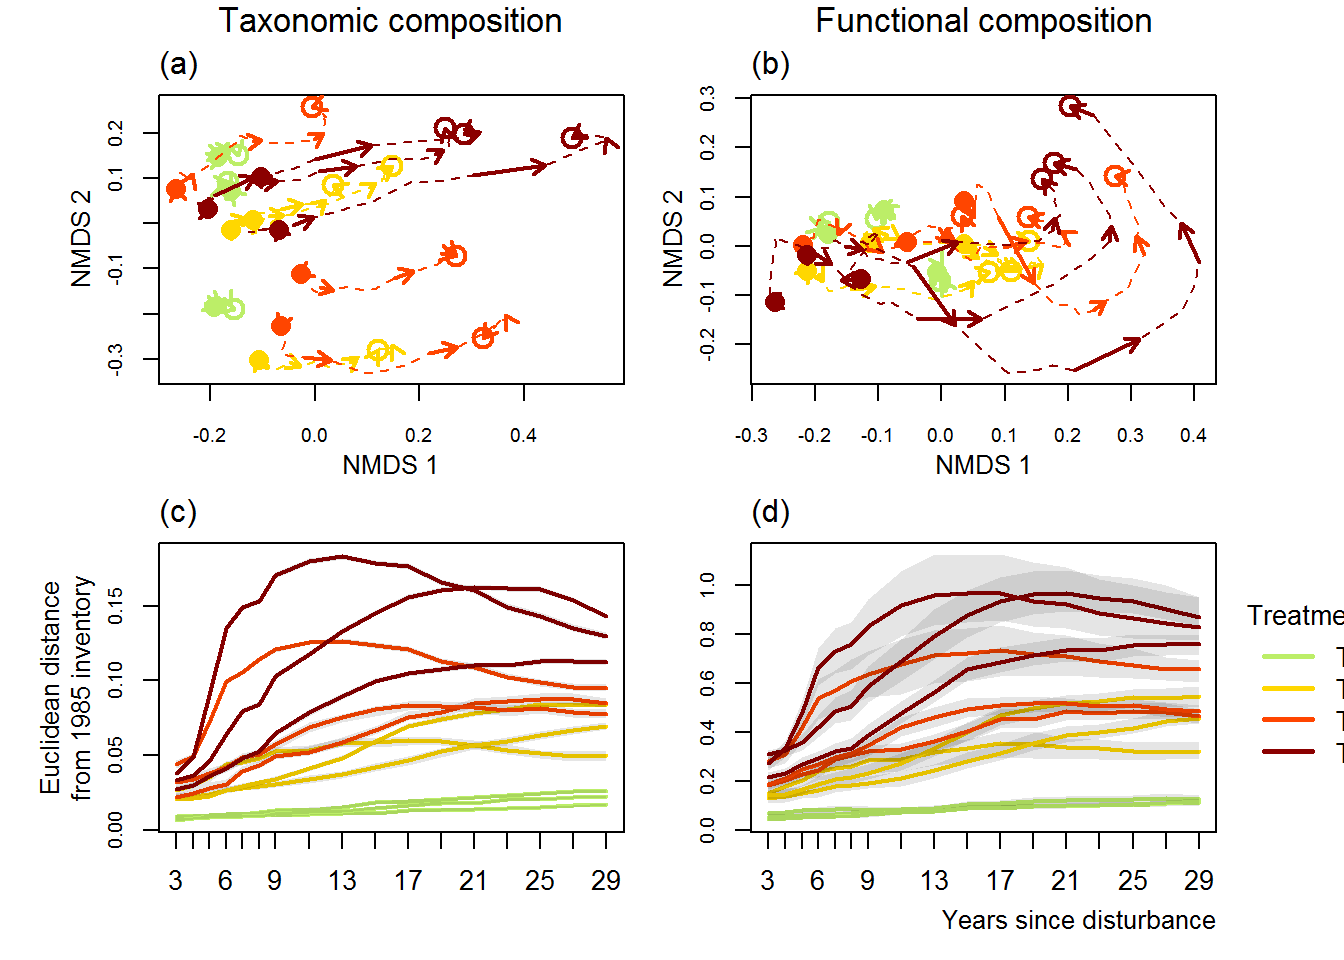
\includegraphics[width=1\linewidth]{WholePlotTrajectories_files/figure-latex/NMDSplans-1} 

}

\caption{Plot trajectories in terms of taxonomic composition (\textbf{(a)} and \textbf{(c)}) and functional composition (\textbf{(b)} and \textbf{(d)}) in a two-dimensional NMDS plane. Lower panels (\textbf{(c)} and \textbf{(d)}) represent the Euclidean distance to initial condition along the 30 sampled years. Shaded areas are the credibility intervals.}\label{fig:NMDSplans}
\end{figure*}

In control plots, Community Weighted Means (CWM) of functional traits
remain stable in time.\\
In disturbed plots, they mostly followed unimodal trajectories, either
stabilizing or returning towards their initial values, to the exception
of leaf chlorophyll content, which continued to increase 30 years after
disturbance for some highly disturbed plots. Maximum height at adult
stage (\emph{Hmax}), leaf toughness and wood specific gravity
(\emph{WSG}) decreased in time and then slightly increased, but remained
significantly lower than their initial value (Fig. \ref{fig:CWM}). Bark
thickness and specific leaf area (\emph{SLA}) both increased in time.
Bark thickness remained substantially high after 30 years, and
\emph{SLA} had almost recovered to its initial value. Whatever the
functional traits, the maximum difference to initial value was highly
correlated to the disturbance intensity. Positive correlations were
observed for Leaf thickness, chlorophyll content, SLA and bark thickness
(\(\rho_{Spearman}^{Leaf thickness}=0.76\),
\(\rho_{Spearman}^{Chlorophyll content}=0.60\),
\(\rho_{Spearman}^{SLA}=0.93\),
\(\rho_{Spearman}^{Bark thickness}=0.71\)). Negative correlation was
observed for Leaf toughness, WSG and Hmax
(\(\rho_{Spearman}^{Leaf toughness}=-0.53\),
\(\rho_{Spearman}^{WSG}=-0.75\), \(\rho_{Spearman}^{Hmax}=-0.40\)) The
proportions of the three lightest seed mass classes increased in all
disturbed plots. After 30 years the proportion of lightest seed mass
class decreased while it stabilized for the two other lightest seed mass
classes (Supp. Mat. - Fig. S2).

\begin{figure*}

{\centering 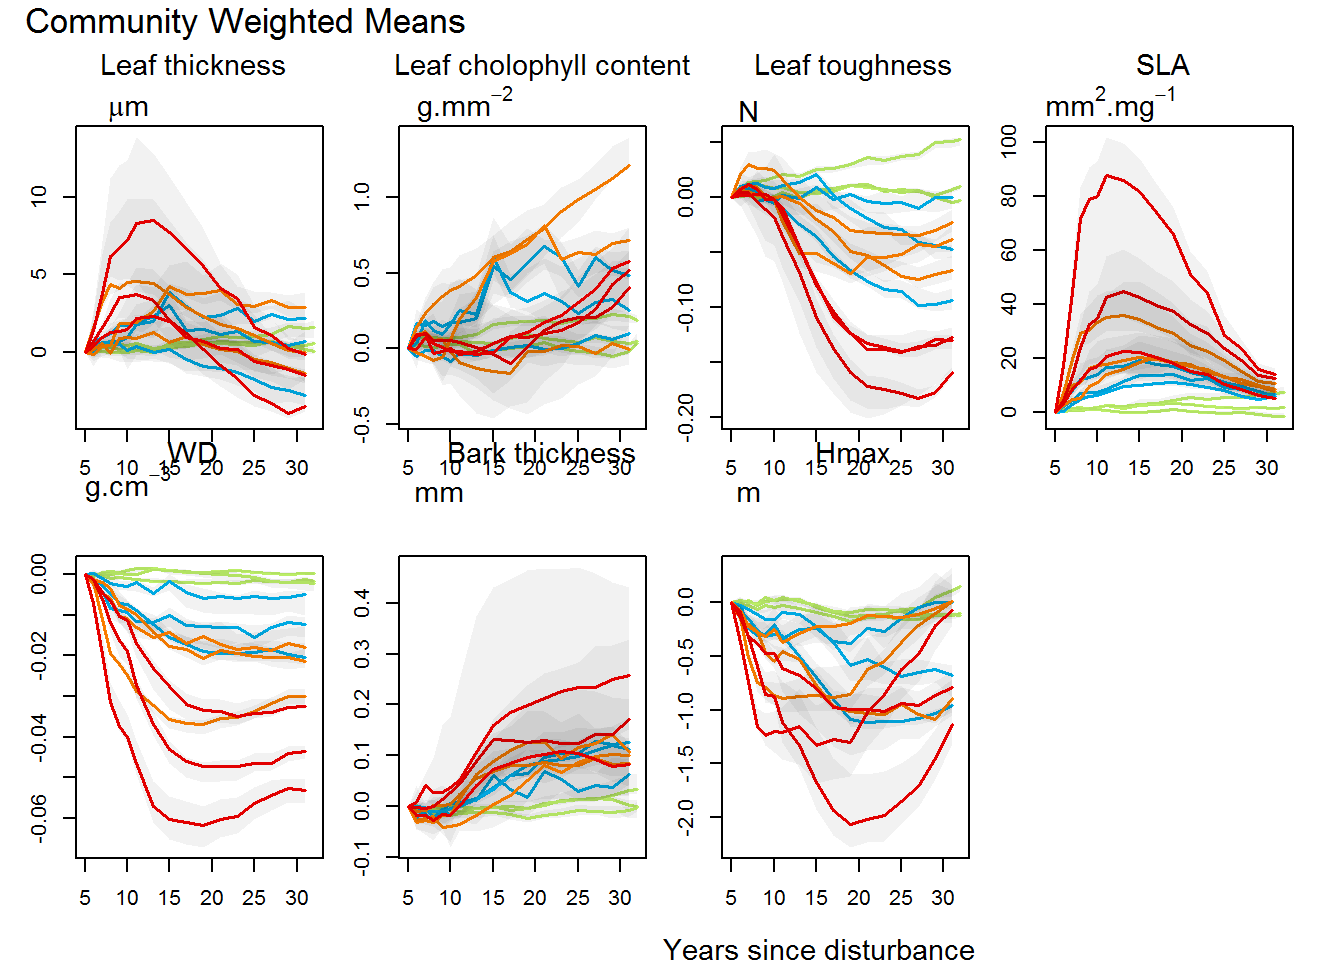
\includegraphics[width=1\linewidth]{WholePlotTrajectories_files/figure-latex/CWM-1} 

}

\caption{Trajectories of community weighted means over 30 years after disturbance of four leaf traits (Leaf thickness, chlorophyll content, toughness, and specific area), two stem traits (wood specific gravity, and bark thickness) and one life history trait (Specific maximum height at adult stage). }\label{fig:CWM}
\end{figure*}

\subsection{Community taxonomic and functional
diversity}\label{community-taxonomic-and-functional-diversity}

Taxonomic richness and evenness remained stable in control plots over
the 30 years of monitoring. In disturbed communities, after low
disturbance intensity the taxonomic richness increased, reaching a
maximum gain of 14 botanical genera. After intense disturbance the
taxonomic richness followed a more complex trajectory, decreasing for
ten years after disturbance before recovering to pre-disturbance values.
The maximum richness loss or gain after disturbance was positively
correlated with the disturbance intensity
(\(\rho_{Spearman}^{Richness}=0.50\)).

In all disturbed plots the evenness first increased until a maximum
reached after around 20 years. This maximum was positively correlated
with the disturbance intensity (\(\rho_{Spearman}^{Simpson}=0.77\)). The
evenness then stabilized except for two intensively-disturbed plots
(number 8 and 12) for which it kept increasing \ref{fig:DivTaxo}).

\begin{figure*}

{\centering 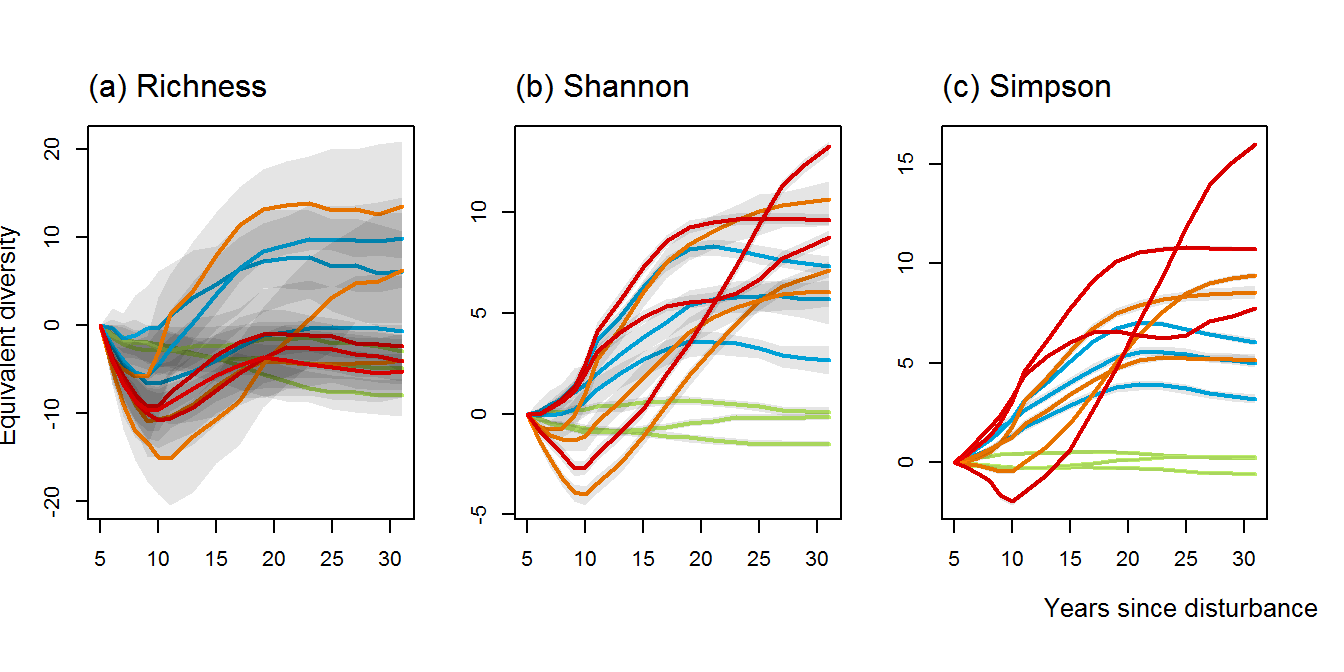
\includegraphics[width=1\linewidth]{WholePlotTrajectories_files/figure-latex/DivTaxo-1} 

}

\caption{Trajectories of community taxonomic richness \textbf{(a)}, Simpson diversity \textbf{(b)}, functional richness \textbf{(c)}, and Rao diversity \textbf{(d)}. Values correspond to the difference over 30 years of community diversity with the values of reference 1984 pre-disturbance inventories. Shaded areas are the credibility intervals }\label{fig:DivTaxo}
\end{figure*}

Functional richness and evenness remained stable in control plots over
the 30 years of monitoring. In disturbed communities, both trajectories
depended on the disturbance intensity, with their maximum values in time
being positively correlated to \%AGB loss
\(\rho_{Spearman}^{Richness}=0.76\) and \(\rho_{Spearman}^{Rao}=0.60\).
Functional richness and evenness displayed for low disturbance intensity
a low but long-lasting increase up to a maximum reached after 20-25
years. For high disturbance intensity, they generally displayed a fast
but short increase followed after 10 years by a slow decrease towards
the initial values.

The second-degree polynomial regressions between (i) the percentage AGB
loss and (ii) the taxonomic and functional diversity showed various
shape depending on the diversity indices and on the time since
disturbance (Fig. \ref{fig:IDHplot}). Regarding taxonomic diversity, the
relationship between disturbance intensity and diversity was more
markedly hump-shaped for richness than for evenness and peaked at 20\%
of initial AGB loss. Regarding functional diversity, the relationship
was almost linear and similar between richness and evenness. Generally,
all relationships were stronger 20 or 30 years after disturbance than
observed for 10 years.

\begin{figure*}

{\centering 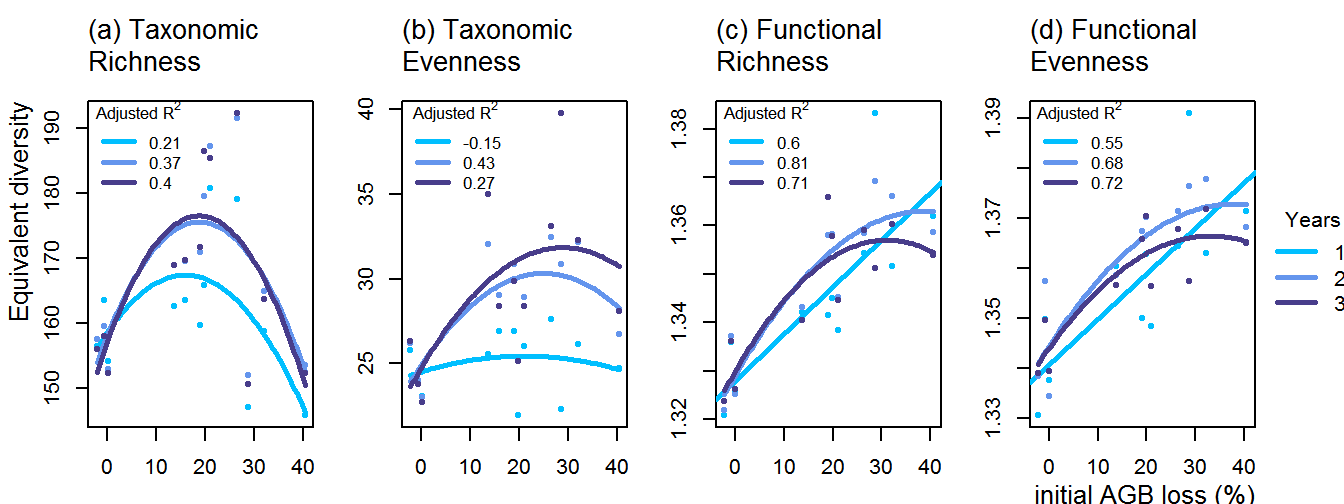
\includegraphics[width=1\linewidth]{WholePlotTrajectories_files/figure-latex/IDHplot-1} 

}

\caption{Relationship between the initial \%AGB loss and community taxonomic richness \textbf{(a)}, taxonomic evenness \textbf{(b)}, functional richness \textbf{(c)},and functional evenness \textbf{(d)} at 10, 20 and 30 years after disturbance}\label{fig:IDHplot}
\end{figure*}

\subsection{Functional redundancy}\label{functional-redundancy}

Control plots displayed stable functional redundancy over time. All
disturbed plots had lower functional redundancy than control plots and
followed similar hump-shaped trajectories (\ref{fig:RedFunRest}). The
maximum redundancy loss was positively correlated with the disturbance
intensity (\(\rho_{Spearman}=0.47\)) and the recovery trajectory had not
attained initial values for any disturbed communities after 30 years.

\begin{figure}

{\centering 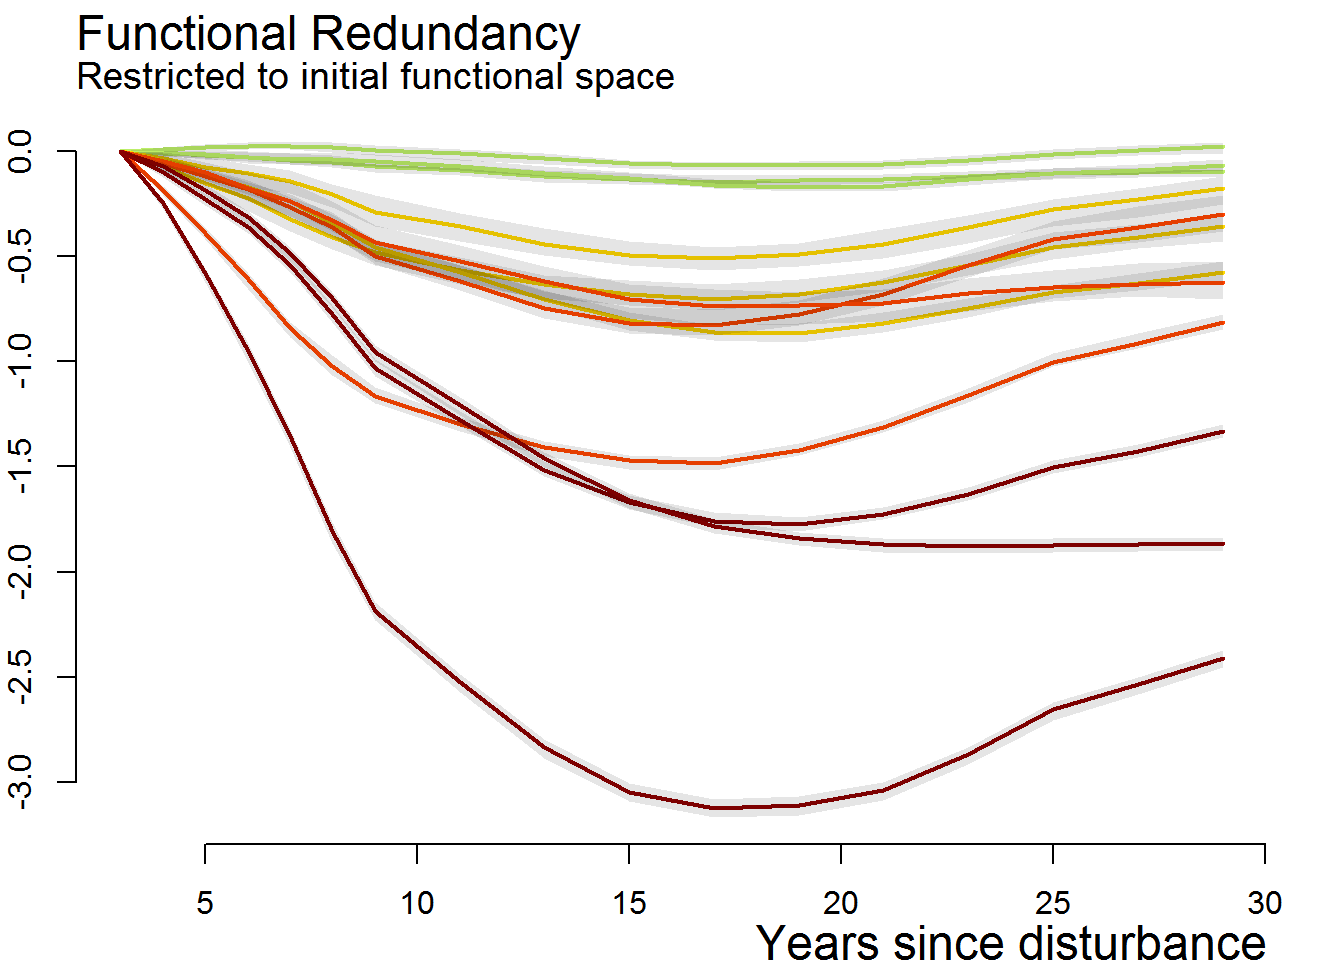
\includegraphics[width=1\linewidth]{WholePlotTrajectories_files/figure-latex/RedFunRest-1} 

}

\caption{Trajectories of the functional redundancy within the initial functional space over 30 years after disturbance. Shaded areas are the credibility intervals.}\label{fig:RedFunRest}
\end{figure}

\section{Discussion}\label{discussion}

Our analysis highlighted the decoupling between functional and taxonomic
trajectories, with taxonomic trajectories maintaining initial
differences among plots while functional trajectories remained similar.
We revealed that if the IDH explained the taxonomic response to
disturbance, it was not validated regarding the functional response. The
decoupling between taxonomic and functional response was linked to the
disturbance impact on the functional redundancy, that proved determining
in community recovery.

\subsection{Decoupled taxonomic and functional
trajectories}\label{decoupled-taxonomic-and-functional-trajectories}

Regarding taxonomic composition, the different tree communities were
substantially different before disturbance, and this is visualized by
their distinct starting points on the NMDS axis 2. These initial
differences were maintained all along the 30 years following
disturbance, with the disturbance leading a displacement on the NMDS
axis 1 only. Changes were thus similar and may correspond to the
recruitment of a group of pioneers, e.g. \emph{Cecropia} spp.,
\emph{Vismia} spp., shared by all plots and whatever their initial
taxonomic differences and the intensity of disturbance
\citep{Denslow2000, Bongers2009}. Taxonomic trajectories seems to start
a recovery to the initial composition which, although far from fully
achieved after 30 years, suggested that taxonomic composition is
resilient and that the initial differences will be maintained in time
\citep{Folke2006}. This would show that species not belonging to the
pre-disturbance community were rarely recruited in the long-term,
probably because of the common dispersal limitations among tropical tree
species \citep{Svenning2005}.

Regarding functional composition, initial communities had similar
starting points and this contrasts to taxonomic composition. This means
that, despite differences in species composition, the functional
signature of the tree communities were quite similar. Following
disturbance, functional trajectories were consistent in the NMDS plane
with displacement intensities linked to disturbance intensities and thus
relied upon the recruitment of a shared pool of functional types
previously infrequent or absent. This common pool is composed of pioneer
resource-acquisitive (low leaf toughness, wood specific gravity, maximum
height and high Specific Leaf area) strategies that translated by a
displacement to the right along the first NMDS axis
\citep{Westoby1998, Wright2004, Reich2014}. Thereafter, the pioneers
recruited primarily were progressively excluded by long-lived, more
competitive and shade-tolerant species. The community functional
composition then quickly returned towards more resource-conservative
strategies, suggesting the recovery of the initial functional
composition. This recovery translated in the functional plane by a
displacement left along the first axis and upward along the second axis
(Fig. \ref{fig:NMDSplans}).

Both taxonomic and functional composition trajectories initiated a
return towards pre-disturbance state after 30 years, which highlighted
the taxonomic and functional resilience of communities. Taxonomic and
functional trajectories however appeared decoupled: while taxonomic
trajectories maintained the initial differences among communities, the
functional trajectories where similar and convergent in the functional
space \citep{Fukami2005} exemplifying the simultaneous operation of
trait-based assembly rules and species-level priority effects that
shapes tree community assembly in this forest, making it both
deterministic in functional space and historically contingent in
taxonomic space.

\subsection{The scope of the intermediate disturbance
hypothesis}\label{the-scope-of-the-intermediate-disturbance-hypothesis}

Community trajectories depended on the disturbance intensity, with a
threshold of 20-25\% of AGB loss for which the taxonomic richness was
maximized and the taxonomic evenness remained resilient. Below a
disturbance intensity threshold (treatments 1 and 2), the taxonomic
richness increased and the taxonomic eveness increased first before
stabilizing or starting to decrease. In those cases, the trees surviving
after disturbance remained numerous enough to maintain the high
taxonomic richness of the pre-disturbance community \citep{Bongers2009}.
In parallel, the recruitment of pioneers, infrequent or absent before
disturbance, increased the taxonomic richness all the more so that the
disturbance was intense \citep{Martin2015, Chaudhary2016}. As these
pioneers became more dominant they balanced the usual hyper-dominance of
tropical forests and increased the taxonomic evenness
\citep{Baraloto2012a}. Contrastingly, above the intensity threshold
(treatment 3), the taxonomic richness did not exceed the initial value
and the taxonomic evenness continuously increased without sign of
reversal. Above the intensity threshold, the taxonomic richness of
surviving trees was too low to be offset by the recruitment of pioneers.
In the Guiana shield indeed, the pool of true pioneers specifically
recruited after disturbance is restricted to a few common genera (e.g.
\emph{Cecropia} spp., \emph{Vismia} spp.) \citep{Guitet2018}. At the
same time, pioneers became persistently dominant and prevented a return
towards the initial evenness and the recovery of hyper-dominant
shade-tolerant species.

After disturbance of intermediate intensity, taxonomic evenness
trajectories were hump-shaped, as already observed in the Guiana shield
\citep{Baraloto2012a} and in Bornean tropical forests
\citep{Cannon1998}. Trajectories peaked at an intermediate time after
disturbance, around 15-20 years. This time corresponded to a balance
between first established pioneers and the more competitve
late-successional species.

Regarding community functional trajectories in contrast, there was
neither intermediate disturbance intensity nor intermediate time after
disturbance, which dismissed the IDH. Neither functional richness nor
functional evenness displayed a humped-shaped pattern, but both rather
increased with the recruitment of pioneers that were functionally highly
different from the pre-disturbance community
\citep{Denslow1980, Molino2001}. Above the intensity threshold however,
for the most intense disturbance, community functional richness and
evenness started to decrease after 15 to 20 years. Right after
disturbance, short-lived species benefited from the resources made
available and prevented the establishment of other species. The decline
of these short-lived pioneers decreased the functional richness and
evenness, but we suggest that the establishment of long-lasting pioneers
will follow and that the trajectories will catch up with those observed
for intermediate disturbance \citep{Walker2009}.

\subsection{The functional redundancy, key of community
resilience}\label{the-functional-redundancy-key-of-community-resilience}

The loss of species following disturbance decreased the functional
redundancy during the first 15 years. Progressively though, the
functional redundancy was restored through the replacement of the
resource-acquisitive strategies species by more late-successional
species that were functionally closer to the pre-disturbance community.
This replacement followed the lottery recruitment rules, implying an
easy recruitment for the first species but becoming increasingly
hampered by the emergence of interspecific competition
\citep{Busing2002} and this explains why the slope of the recovery
trajectory became less and less significant 20 years after disturbance.
The recovery of the functional redundancy then relied upon the random
process of species recruitment and was increasingly slow and difficult
to anticipate \citep{Elmqvist2003, Diaz2005}. This suggests a low
resilience of the functional redundancy with the random recovery of
infrequent species increasing the risks to lose keystone species, with
unexpected ecological consequences
\citep{Jones1994, Chazdon2003a, Diaz2005}. Infrequent species might
indeed have unique functional characteristics, apart from those
considered here, in the ecosystem or be a key resource for some fauna
\citep{Schleuning2016}.

\section{Conclusion}\label{conclusion}

Post-disturbance trajectories of tree community composition and
diversity were both shaped by the recruitment of a determined pool of
pioneers identical among local communities and independent of the
disturbance intensity. (i) Composition trajectories in taxonomic and
functional space nevertheless appeared decoupled. While functional
trajectories remained similar in the functional space and converged
towards the recovery of a comparable initial state, taxonomic
trajectories showed initial differences in community composition that
were maintained along time. Community high functional redundancy
mediated this decoupling, as the loss of a species does not necessarily
entails the loss of its functional charactristics. (ii) Diversity
trajectories were contrasted as well. While the functional trajectories
remained similar whatever the disturbance intensity, taxonomic
trajectories were markedly different with a threshold at 20-25\% AGB
removed for which taxonomic richness was maximized. The Intermediate
Disturbance Hypothesis applied well to taxonomic diversity, but not to
the functional diversity. Taxonomic diversity was maximized at an
intermediate time after disturbance, that was around 25 years after
disturbance when the recruitment of early- and late-successional species
were balanced. Whenever the disturbance intensity, community resilience
(in terms of recovery of the pre-disturbance state) was tangible but
required several decades and relied upon the random lottery recruitment
of rare species. Given the long-term impacts of disturbance observed, we
suggest that 30 years is not enough time for tropical communities to
recover, even after relatively low intensity disturbance. Much of
community response to disturbance rely on species recruitment: refined
understanding of post-disturbance trajectories would be given by a
closer analysis of recruitment processes.

\section{Acknowledgement}\label{acknowledgement}

We are in debt with all technicians and colleagues who helped setting up
the plots and collecting data over years. Without their precious work,
this study would have not been possible and they may be warmly thanked
here.

\section{Author's contributions}\label{authors-contributions}

AM, EM \& BH designed the study, developed the analysis framework and
interpreted the results. AM wrote the manuscript with contributions by
EM \& BH. All authors gave final approval for publication.

\section{Data availability}\label{data-availability}

This article is based upon the dataset of the Paracou station, which is
part of the Guyafor permanent plot network in French Guiana
(Cirad-CNRS-ONF). The dataset is available upon request to the
scientific director (https://paracou.cirad.fr).

%----------------------------------------------------------------------------------------
%	REFERENCE LIST
%----------------------------------------------------------------------------------------

\bibliographystyle{mee}
\makeatletter
% The filename has .bib extension the must be eliminated
\filename@parse{references.bib}
% parse stores the file name in base. Extension starts at the first dot, so don't use dots in file names.
\bibliography{\filename@base}
\makeatother


%----------------------------------------------------------------------------------------

\end{document}
